%% LyX 2.2.0alpha2 created this file.  For more info, see http://www.lyx.org/.
%% Do not edit unless you really know what you are doing.
\documentclass[english]{article}
\usepackage[T1]{fontenc}
\usepackage[latin9]{luainputenc}
\usepackage{geometry}
\geometry{verbose,tmargin=3cm,bmargin=3cm,lmargin=3cm,rmargin=3cm}
\usepackage{graphicx}
\usepackage{esint}

\makeatletter
%%%%%%%%%%%%%%%%%%%%%%%%%%%%%% User specified LaTeX commands.
\usepackage{fancyheadings}
\pagestyle{fancy}
\lhead{Kellen Betts}
\chead{frequencyTracking}
\rhead{160731}

\makeatother

\usepackage{babel}
\begin{document}

\title{Frequency Tracking}

\author{Kellen Betts}

\date{Updated July 31, 2016}
\maketitle
\begin{abstract}
The objective of this project is to identify a frequency signature
in highly noisy data and track its movement in time and space. Standard
time-frequency methods are used including the Fast Fourier Transform
(FFT), temporal averaging, and a Gaussian filter. The FFT is used
to obtain the spectral content of the data. A frequency signature
is isolated in the data by averaging out the noise across twenty time
points. The frequency signature is then used in the Gaussian filter
to identify its location at each time point and track its movement.
\end{abstract}

\section{Introduction}

The setup for this problem involves my poor dog Fluffy swallowing
a marble, going to the vet to get an ultrasound, and saving Fluffy
by locating the marble in the ultrasound data. The given data is three
dimensional in space and evolves over 20 samples in time. Fluffy's
movement and the intestinal environment have generated highly noisy
data and caused the marble to move in both space and time, so time-frequency
filtering methods are the key finding its location. We are asked to
provide: (1) the marble's frequency signature, (2) the marble's path,
and (3) the marble's final location so the vet can use an intense
acoustic wave to break it up.

\section{Theoretical Background}

To isolate the frequency signature and track its movement, standard
time-frequency analysis techniques are used including the Fast Fourier
Transform, temporal averaging, and a Gaussian filter. The Fourier
series is used as the basis for the spectral content in the data.
For a given function $f(x)$ the Fourier Transform and its inverse
are defined as,
\begin{equation}
F\left(k\right)=\frac{1}{\sqrt{2\pi}}\intop_{-\infty}^{\infty}e^{-ikx}f\left(x\right)dx
\end{equation}
\begin{equation}
f(x)=\frac{1}{\sqrt{2\pi}}\intop_{-\infty}^{\infty}e^{ikx}F(k)dk
\end{equation}
where $k$ corresponds to the wavenumbers in the trigonometric identity.
Computationally the transform is implemented over a finite domain
$x\,\epsilon\,\left[-L,L\right]$ using the Fast Fourier Transform
(FFT). One of the important advantages of the FFT algorithm is the
low operation count of $O\left(N\,\log N\right)$ using a $2^{n}$
discritization. Additionally, given its trigonometric construction,
the transform assumes a $2\pi$-periodic domain.

To isolate the marble's frequency signature, the random nature of
the noise is exploited by averaging across repeated samples where
the mean for random noise is approximately zero. Once the frequency
signature is isolated, the path of the marble is identified by filtering
each time step with a Gaussian filter defined as,
\begin{equation}
\mathcal{F}\left(k\right)=\exp\left(-\tau\left(k-k_{0}\right)\right)
\end{equation}
where $\tau$ is the bandwidth, $k$ is the wavenumber, and $k_{0}$
is the center frequency determined in the averaging process. 

\section{Algorithm Implementation and Development}

There are three essential steps in the solution to this problem: (1)
initialization of data and variables, (2) identification of the marble's
frequency signature by averaging across the temporal domain, and (3)
filtering each time point to track the marble's path through time.
Most of the parameters are given in the project description. Discritization
is set at $n=64$ with the spatial domain defined over $x,y,z\,\epsilon\,\left[-15,15\right]$.
The spatial domain is discritized with $n+1$ points then trimmed
to $n$ points since the FFT assumes periodic boundaries. The frequency
domain is discritized using, 
\begin{equation}
\mathtt{k=\frac{2\pi}{2L}\left[0:(\frac{n}{2}-1)-\frac{n}{2}:-1\right]}
\end{equation}
which aligns with the shifted and $2\pi$-scaled domain of the FFT
algorithm. The $\mathtt{x,y,z}$ and $\mathtt{k}$ vectors are then
mapped to $n\times n\times n$ matrices to match the three-dimensional
dataset.

The second critical step in the algorithm is isolating the marble's
frequency signature by averaging the spectral content in the data
across the temporal domain. The original data contains 20 time points
in a $20\times n^{3}$ matrix with each row corresponding to a single
sample (specific spatial/temporal scale and units are not given).
Averaging is implemented by looping through each sample. The incoming
data is . Inside the loop a given sample is reshaped to a $n\times n\times n$
matrix then transformed into the frequency domain using the FFT. The
transformed sample is then added to a running sum. After the loop
runs through all 20 samples, the absolute value of the running sum
is averaged over for the 20 samples. Since the mean of random noise
is approximately zero, the frequency signature is isolated by finding
the maximum value in the data. More specifically, the index of the
maximum is used to find the corresponding wavenumber $\left(k_{0}\right)$
which is need for the Gaussian filter. To confirm the frequency signature,
the averaged data is plotted mindful of the need to shift the data
since it is in the FFT domain.

Once the frequency signature is isolated, the final step in the algorithm
involves filtering each time step independently to track the marble's
path and find its final location. Filtering is done in a loop that
reshapes a given sample into a $n\times n\times n$ matrix and passes
it through the FFT. Once in the frequency domain, the data gets multiplied
by the Gaussian filter effectively denoising the sample around the
center frequency. The marble's location is identified as before by
finding the index of the maximum value then using the index to map
the specific $x,y,z$ coordinates. Since the marble is moving in time
and space, the coordinates are logged for each sample. To confirm
the marble's path, each filtered sample is plotted and overlaid with
the final plot of the path. 

\section{Computational Results}

By averaging the data across the 20 samples, the wavenumbers corresponding
to the marble's \emph{frequency signature} are $\left(1.8850,\,-1.0472,\,0\right)$
or approximately $\left(2,\,-1,\,0\right)$. This is confirmed in
the plots of the averaged data (shifted and normalized) as seen in
Figure 1. 

For the Gaussian filter different values of the bandwidth $(\tau)$
were tested, but the results were similar for $0.1<\tau<1$. The \emph{marble's
path} is a downward, counterclockwise spiral starting at approximately
$\left(4.7,\,-4.7,\,9.9\right)$ and ending at the\emph{ final location}
of $\left(-5.6250,\,4.2188,\,-6.0938\right)$. A plot of the path
overlaid with the surface plots for each time step can be seen in
Figure 2. Most importantly, the vet should direct the intense acoustic
wave at approximately $\left(-5.6,\,4.2,\,-6.1\right)$ to blast the
marble and save Fluffy!

\pagebreak{}

\noindent \begin{center}
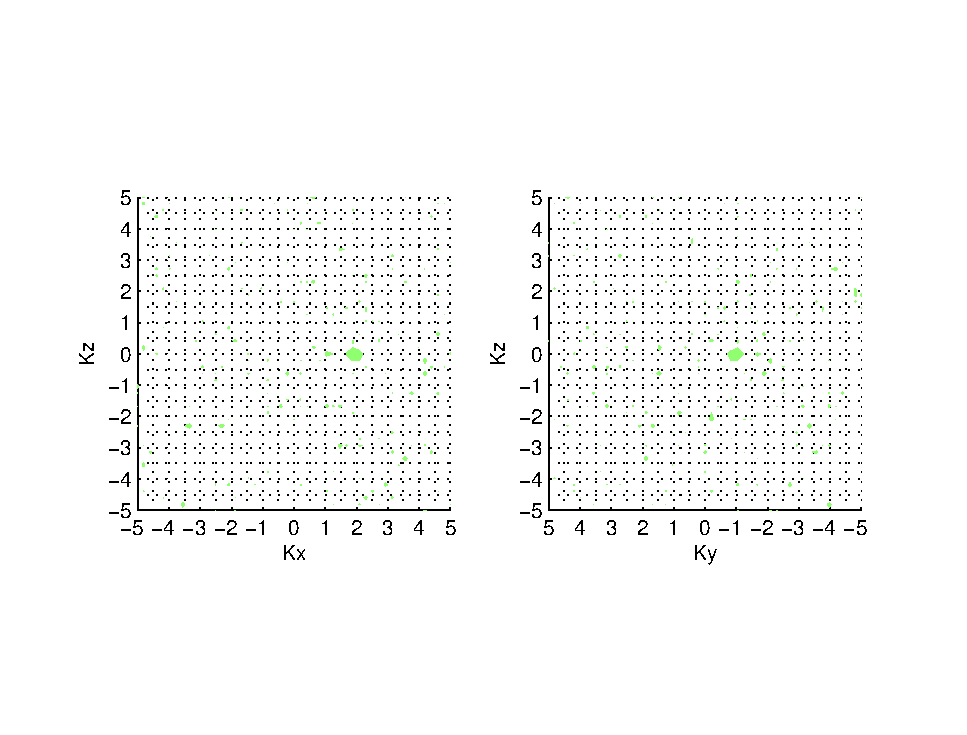
\includegraphics[width=0.85\columnwidth]{plots/averaged}\textbf{}\\
\textbf{}%
\begin{minipage}[t]{0.75\columnwidth}%
\textbf{Figure 1.} Plot of the 3D frequency data denoised by averaging
across 20 time steps. The data is shifted and normalized, and the
plot views are set to the X-Z (left) and Y-Z (right) planes. The green
sphere located at approximately $\left(2,\,-1,\,0\right)$ is the
marble's frequency signature.%
\end{minipage}
\par\end{center}

\vspace{0.1\paperheight}

\noindent \begin{center}
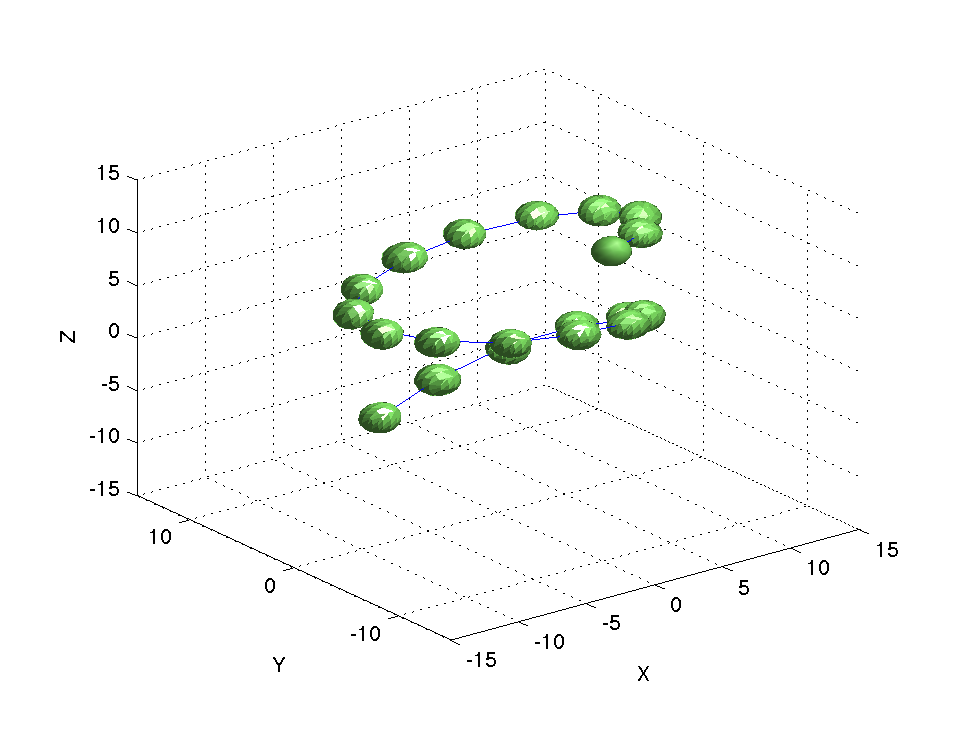
\includegraphics[width=0.75\columnwidth]{plots/overlay}\textbf{}\\
\textbf{}%
\begin{minipage}[t]{0.75\columnwidth}%
\textbf{Figure 2.} Plot of the marble's path through time. Each green
sphere corresponds to a single time step. The path is a downward,
counterclockwise spiral starting at $\sim\left(4.7,\,-4.7,\,9.9\right)$
and ending at $\sim\left(-5.6,\,4.2,\,-6.1\right)$.%
\end{minipage}
\par\end{center}

\pagebreak{}

\section{Summary and Conclusions}

Ultimately, this project demonstrates that standard time-frequency
methods such as the FFT, temporal averaging, and a Gaussian filter
can be used to isolate a frequency signature in highly noisy data
and track its movement time and space. The FFT algorithm is a critical
computational element used to solve this problem, and having it provided
as a built-in MATLAB function greatly simplifies the programming process.
One aspect of this algorithm that proved challenging was isolating
the index of the maximum value in the data. The incoming data is in
three dimensions, but the $\mathtt{max}$ and $\mathtt{find}$ MATLAB
functions provide a linear index (data is stacked to $1\times n^{3}$).
The documentation for the $\mathtt{find}$ function suggests using
the $\mathtt{ind2sub}$ function to convert the linear index to the
corresponding matrix subscripts but the results I initially got from
this were incorrect (did not match the plot). Fortunately, one of
my classmates posted the suggestion on the discussion board that $\mathtt{ind2sub}$
does not output $x,y$ indices in the order that correspond to the
original data so they needed to be swapped. This insight was very
helpful and I am indebted to their contribution on the discussion
board.

\section*{Appendix A (Functions)}
\begin{description}
\item [{abs}] Takes the absolute value.
\item [{fftn}] The all important FFT function, which performs a discritized
Fourier Transforms. This version of the function transforms $n$-dimensional
data. The $\mathtt{fft}$ and $\mathtt{fft}2$ versions transform
1- and 2-dimensional data respectively.
\item [{fftshift}] The output of the $\mathtt{fft}$ algorithm is shifted
(butterfly algorithm), so data in the frequency domain is shifted
back using this function before plotting.
\item [{ind2sub}] This function proved highly useful and problematic. It
is used to convert the linear index of the maximum value in the data
(pulled from the $\mathtt{max}$ function) into the corresponding
3D matrix subscripts. As described in\emph{ }Summary and Conclusions,
the output from this function did not match the $x,y$ spatial relation
in the original data and so the coordinates need to be swapped. This
was suggested by a classmate, and confirmed by plotting the data and
by digging through the function's documentation.
\item [{isosurface}] Used to plot 3D surfaces to visualize the marble's
frequency signature in the averaged data and its location at each
time step in the filtered data.
\item [{linspace}] Used to build a linear vector with $n+1$ points for
the spatial domain. The vector is then trimmed to $n$ points due
to the periodic boundaries.
\item [{max}] Used to find the maximum value and corresponding linear index
in the data. The linear index is then converted to the corresponding
matrix subscripts using $\mathtt{ind2sub}$.
\item [{meshgrid}] Used to build 3D grids from the linear $x,y,z$ and
$k$ vectors.
\item [{plot3}] Used to plot the 3D path of the marble using the coordinates
obtained at each time step.
\item [{reshape}] Used to covert vectors (i.e. $1\times n^{3}$) to matrices
(i.e. $n\times n\times n$) and back.
\item [{size}] Used to get the number of rows (time steps) in the original
data. This generalizes the script allowing a larger dataset to be
implemented more easily.
\item [{zeros}] Used to build vectors and matrices filled with zeros.
\end{description}

\section*{Appendix B (Code)}

See project root for files.
\end{document}
